% Compilar con: pdflatex Informe_Divulgativo_Laboratorio_2_10_Paginas.tex
% Documento diseñado para producir exactamente 10 páginas.
\documentclass[10pt,letterpaper]{article}

\usepackage[utf8]{inputenc}
\usepackage[T1]{fontenc}
\usepackage{lmodern}
\usepackage{microtype}
\usepackage[letterpaper,margin=1.65cm,headheight=14pt,footskip=22pt]{geometry}
\usepackage{graphicx}
\usepackage{xcolor}
\usepackage{booktabs}
\usepackage{array}
\usepackage{tabularx}
\usepackage{enumitem}
\usepackage{fancyhdr}
\usepackage{titlesec}
\usepackage{hyperref}
\usepackage{lastpage}

\definecolor{Navy}{HTML}{102A43}
\definecolor{Blue}{HTML}{176B87}
\definecolor{Teal}{HTML}{2A9D8F}
\definecolor{Cyan}{HTML}{2E86AB}
\definecolor{Gold}{HTML}{E9A23B}
\definecolor{Red}{HTML}{D95D39}
\definecolor{Ink}{HTML}{183247}
\definecolor{Soft}{HTML}{F2F7FA}
\definecolor{SoftGreen}{HTML}{EAF8F4}
\definecolor{SoftGold}{HTML}{FFF5DF}
\definecolor{Line}{HTML}{D5E3EB}

\hypersetup{
  colorlinks=true,
  linkcolor=Blue,
  urlcolor=Cyan,
  pdftitle={Laboratorio 2 - Informe para público general},
  pdfauthor={Jorge Gabriel Palacios Sales, Pablo Daniel Barillas Moreno y Roberto Emiliano Otoniel Camposeco Torres}
}

\pagestyle{fancy}
\fancyhf{}
\fancyhead[L]{\small\color{Navy}\textbf{Visitantes internacionales y predicción}}
\fancyhead[R]{\small\color{Navy}Informe para público general}
\fancyfoot[C]{\small Página \thepage\ de \pageref{LastPage}}
\renewcommand{\headrulewidth}{0.35pt}
\renewcommand{\footrulewidth}{0pt}

\titleformat{\section}
  {\LARGE\bfseries\color{Navy}}
  {}{0pt}{}
  [\vspace{2pt}\color{Line}\titlerule]
\titleformat{\subsection}
  {\large\bfseries\color{Blue}}
  {}{0pt}{}

\setlength{\parindent}{0pt}
\setlength{\parskip}{5pt}
\setlist[itemize]{leftmargin=1.5em,itemsep=2pt,topsep=3pt}
\setlist[enumerate]{leftmargin=1.7em,itemsep=2pt,topsep=3pt}
\graphicspath{{figuras/}}

\newcommand{\callout}[2]{%
  \begin{center}
  \fcolorbox{#1}{Soft}{%
    \begin{minipage}{0.92\textwidth}
    \vspace{4pt}#2\vspace{4pt}
    \end{minipage}}
  \end{center}
}

\newcommand{\plainterm}[2]{%
  \textbf{\color{Blue}#1:} #2
}

\begin{document}

% ---------------------------------------------------------------------------
% PÁGINA 1
% ---------------------------------------------------------------------------
\begin{titlepage}
\pagecolor{Navy}
\color{white}
\vspace*{0.8cm}

{\Large\bfseries UNIVERSIDAD GALILEO\par}
\vspace{0.25cm}
{\large Facultad de Ingeniería\par}
{\large Departamento de Ciencias de la Computación\par}

\vfill

{\color{Teal}\rule{\textwidth}{3pt}}\par
\vspace{0.55cm}
{\Huge\bfseries Laboratorio 2\par}
\vspace{0.2cm}
{\LARGE Predicción de visitantes internacionales\par}
\vspace{0.45cm}
{\Large Informe explicado para público general\par}
\vspace{0.55cm}
{\color{Teal}\rule{\textwidth}{3pt}}\par

\vfill

\begin{tabular}{@{}>{\bfseries}p{3.7cm}p{11cm}@{}}
Curso: & CC3084 - Data Science, sección 11\\[4pt]
Docente: & García Pérez, Lynette\\[4pt]
Integrantes: &
Jorge Gabriel Palacios Sales\\
& Pablo Daniel Barillas Moreno\\
& Roberto Emiliano Otoniel Camposeco Torres\\[4pt]
Datos: & Ingresos mensuales de visitantes a Guatemala,
enero de 2009 a junio de 2026\\
\end{tabular}

\vfill

{\large Guatemala, julio de 2026\par}
\end{titlepage}
\nopagecolor
\color{Ink}
\pagenumbering{arabic}
\setcounter{page}{2}

% ---------------------------------------------------------------------------
% PÁGINA 2
% ---------------------------------------------------------------------------
\section{¿De qué trata este trabajo?}

Cada mes, miles de personas cruzan las fronteras de Guatemala como turistas o
excursionistas. Este laboratorio buscó responder una pregunta práctica:
\textbf{¿se puede anticipar, con base en el historial, cuántos visitantes
llegarán en los próximos meses?} Contar con una respuesta razonable ayuda a
planear personal en fronteras y aeropuertos, coordinar transporte, dimensionar
la promoción turística y anticipar la capacidad de atención necesaria.

Para responder, se trabajó con una base de \textbf{161,036 registros} que
cubre \textbf{210 meses seguidos}, de enero de 2009 a junio de 2026, sin
huecos ni valores imposibles en la variable principal.

\subsection{¿Qué personas se contabilizan?}

La base distingue dos tipos de visitante, y ambos se sumaron para este
análisis:

\begin{itemize}
  \item \textbf{Turistas}: se quedan en el país al menos una noche.
  \item \textbf{Excursionistas}: entran y salen el mismo día.
\end{itemize}

Se dejó fuera la categoría ``Viajero'' porque agrupa cruces que no siempre son
turísticos, y porque la forma de registrarla cambió a partir de 2023, lo que
la haría poco comparable con años anteriores.

\subsection{Las dos series que se pronosticaron}

\begin{tabularx}{\textwidth}{>{\bfseries\color{Blue}}p{3.3cm}X}
\toprule
Total nacional & La suma de todos los turistas y excursionistas que
ingresaron por cualquier frontera del país en cada mes.\\
\addlinespace
01 La Aurora & Solamente quienes llegaron por el principal aeropuerto
internacional.\\
\bottomrule
\end{tabularx}

\callout{Teal}{%
\textbf{Regla que se respetó en todo el trabajo.} Ningún modelo tuvo acceso a
información del futuro. Para estimar un mes determinado, únicamente se usó lo
ocurrido antes de ese mes.
}

\subsection{Un quiebre que marcó la serie}

La pandemia interrumpió los viajes de forma abrupta durante 2020 y 2021, y eso
dejó una cicatriz difícil de modelar: no existía en el historial ningún
cierre de magnitud comparable del cual aprender, así que los modelos tuvieron
que enfrentar un tramo sin precedente directo.

\newpage

% ---------------------------------------------------------------------------
% PÁGINA 3
% ---------------------------------------------------------------------------
\section{¿Cómo se aseguró una prueba justa?}

Los 210 meses se respetaron en su orden cronológico; en ningún momento se
usaron meses futuros para ``adivinar'' meses pasados.

\begin{itemize}
  \item \textbf{Entrenamiento}: 147 meses, de enero de 2009 a marzo de 2021.
  \item \textbf{Prueba final}: 63 meses, de abril de 2021 a junio de 2026.
\end{itemize}

\begin{center}
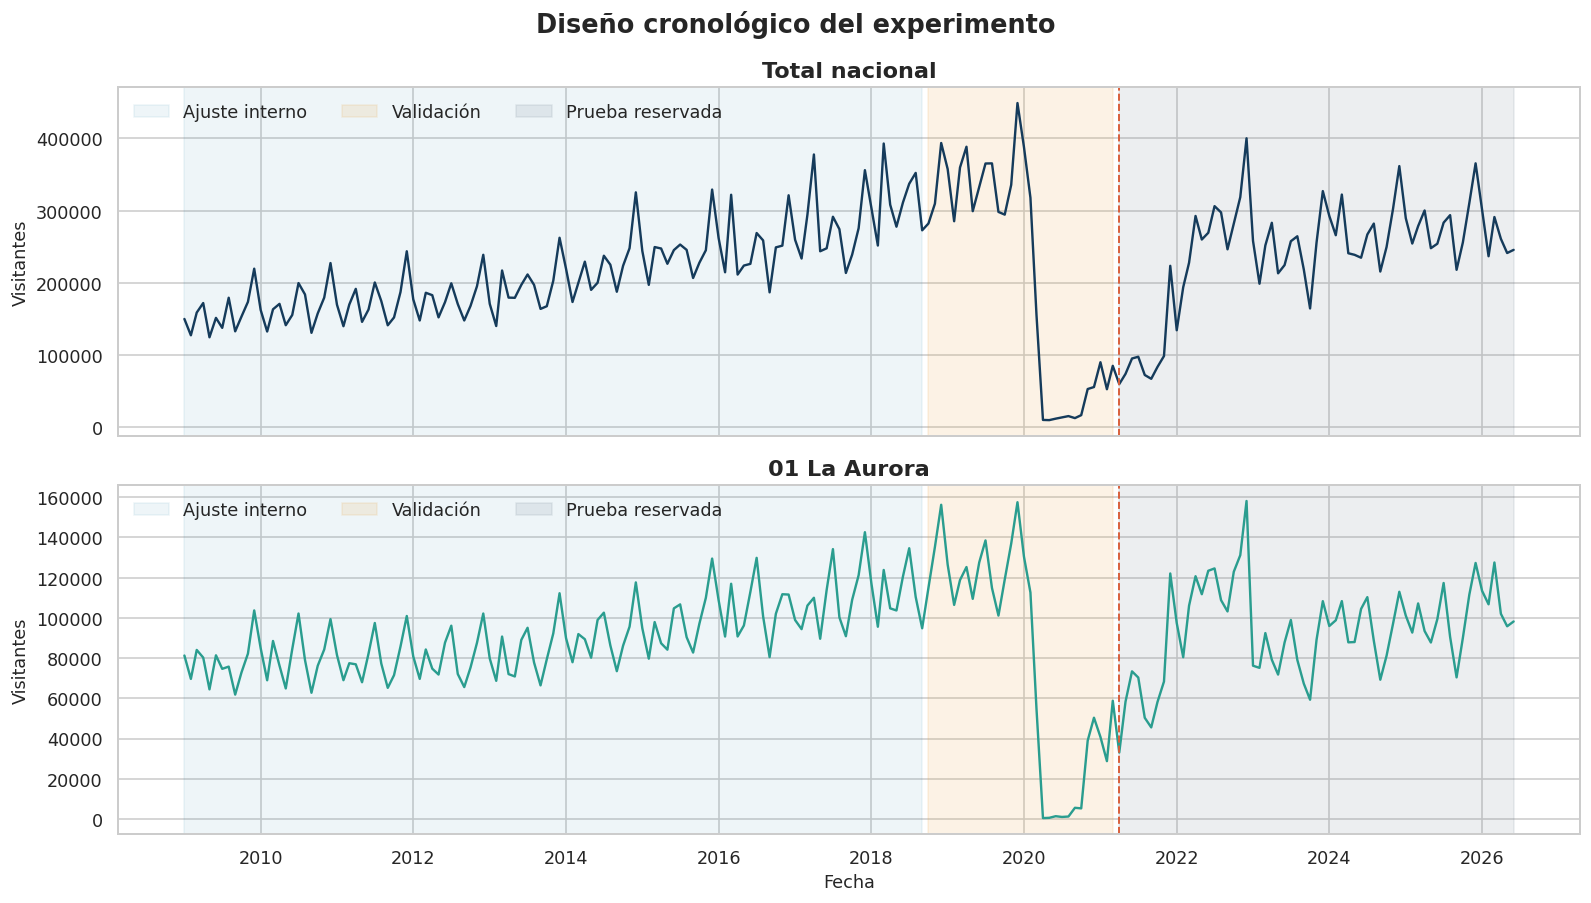
\includegraphics[width=0.92\textwidth]{particion_cronologica.png}
\end{center}

Dentro de los 147 meses de entrenamiento se apartó, además, un tramo interno
para decidir cuál configuración de modelo convenía usar. La comparación es
similar a resolver guías de práctica antes del examen: esas guías permiten
ajustar la estrategia, pero las respuestas del examen final se mantienen
guardadas hasta el final.

\subsection{¿Qué es una ``ventana'' de meses?}

Antes de estimar un mes, el modelo revisa una cantidad fija de meses previos.
Se probaron dos tamaños de ventana:

\begin{itemize}
  \item 12 meses (un año de historia reciente).
  \item 24 meses (dos años de historia reciente).
\end{itemize}

\subsection{¿Con qué se midió el acierto?}

Se calcularon tres indicadores de error, y el más usado para decidir entre
modelos fue el RMSE.

\begin{itemize}
  \item \plainterm{MAE}{el error promedio, expresado directamente en número
  de visitantes.}
  \item \plainterm{RMSE}{parecido al MAE, pero castiga con más fuerza los
  errores grandes.}
  \item \plainterm{sMAPE}{expresa el error como porcentaje, lo que permite
  comparar series de tamaños distintos entre sí.}
\end{itemize}

\callout{Gold}{%
\textbf{Regla de lectura.} En los tres indicadores anteriores aplica lo
mismo: \textbf{mientras más bajo el número, más cerca estuvo el modelo de lo
que realmente ocurrió}.
}

\newpage

% ---------------------------------------------------------------------------
% PÁGINA 4
% ---------------------------------------------------------------------------
\section{¿Qué es una LSTM y cómo se eligió una?}

Una LSTM es una técnica pensada para aprender de datos que llegan en orden,
como los meses de una serie de tiempo. Puede pensarse como una memoria que,
mes a mes, resuelve tres preguntas:

\begin{enumerate}
  \item ¿qué información pasada vale la pena conservar?
  \item ¿qué información reciente conviene incorporar?
  \item ¿qué parte de todo lo anterior se usa para calcular la siguiente
  estimación?
\end{enumerate}

Nadie le indicó a mano cuánto debía subir o bajar la cifra cada mes: el propio
método ajustó sus parámetros internos revisando muchos ejemplos históricos.

\subsection{No se apostó a una sola configuración}

Para no depender de una única receta, se entrenaron y compararon cuatro
variantes de LSTM por cada serie:

\begin{tabularx}{\textwidth}{lXcc}
\toprule
\textbf{Modelo} & \textbf{Estructura} & \textbf{Meses observados} &
\textbf{Tamaño interno}\\
\midrule
LSTM-1A & Una capa de memoria & 12 & 8\\
LSTM-1B & Una capa de memoria & 24 & 16\\
LSTM-2A & Dos capas de memoria & 12 & 12 y 6\\
LSTM-2B & Dos capas de memoria & 24 & 16 y 8\\
\bottomrule
\end{tabularx}

\begin{center}
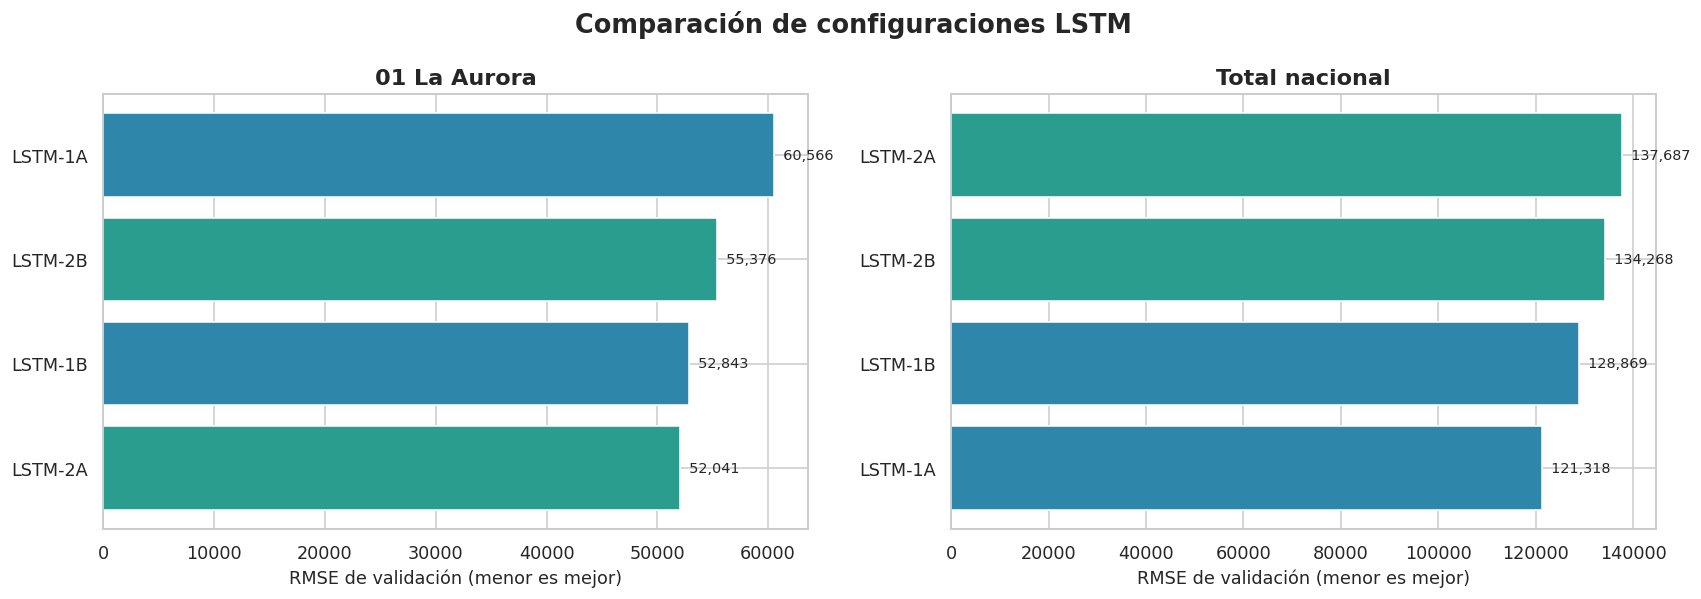
\includegraphics[width=0.93\textwidth]{comparacion_configuraciones.png}
\end{center}

\subsection{Los candidatos que quedaron mejor posicionados}

\begin{itemize}
  \item Para el \textbf{total nacional}, la variante ganadora fue LSTM-1A.
  \item Para \textbf{La Aurora}, la variante ganadora fue LSTM-2A.
\end{itemize}

Vale la pena notar que la red más grande no fue la mejor en ambos casos. Eso
confirma algo importante: agregar más complejidad no garantiza más precisión.
Cuando la cantidad de datos disponibles es limitada, una estructura más
sencilla puede generalizar mejor que una elaborada.

\newpage

% ---------------------------------------------------------------------------
% PÁGINA 5
% ---------------------------------------------------------------------------
\section{El resultado que más importa: la comparación final}

Los dos modelos ganadores se volvieron a entrenar, esta vez con los 147 meses
completos, y produjeron un pronóstico mes a mes para los 63 meses de prueba
que nunca habían visto. Ese pronóstico se comparó contra los mejores modelos
tradicionales obtenidos en el Laboratorio 1.

\begin{center}
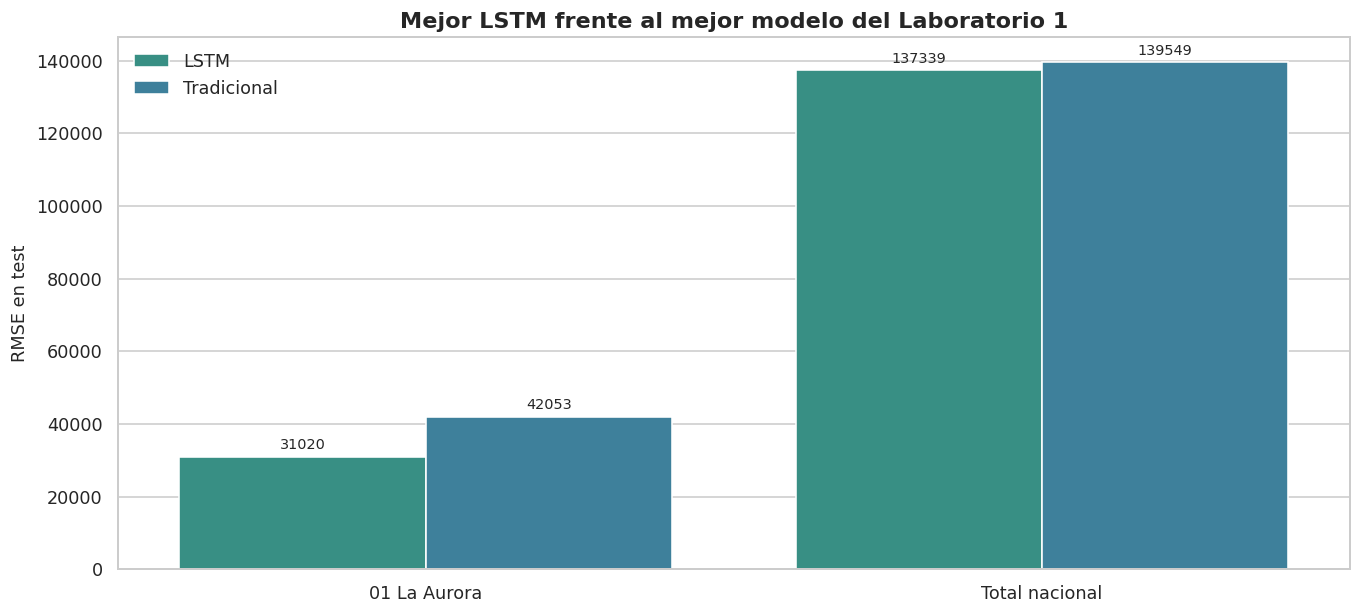
\includegraphics[width=0.88\textwidth]{comparacion_lab1.png}
\end{center}

\begin{tabularx}{\textwidth}{Xrrr}
\toprule
\textbf{Serie} & \textbf{RMSE LSTM} & \textbf{RMSE anterior} &
\textbf{Mejora}\\
\midrule
01 La Aurora & 31,020 & 42,053 & \textbf{26.24\%}\\
Total nacional & 137,339 & 139,549 & \textbf{1.58\%}\\
\bottomrule
\end{tabularx}

\subsection{Cómo interpretar esta tabla}

\textbf{La Aurora.} Aquí la LSTM sí marcó una diferencia clara: su error
grande típico (RMSE) bajó cerca de una cuarta parte frente al método anterior,
llamado SES.

\textbf{Total nacional.} La LSTM también quedó por encima de Prophet, pero por
un margen pequeño, de apenas 1.58\%. En la práctica, esto quiere decir que
ambos métodos tuvieron un desempeño bastante parejo, y que descartar Prophet
por completo no estaría justificado.

\callout{Teal}{%
\textbf{Una conclusión con matices.} La LSTM ganó en estas dos comparaciones
puntuales, pero eso no debe leerse como que siempre será la mejor opción para
cualquier otra frontera, país o período de tiempo.
}

Que ambas series se comporten distinto tiene sentido: La Aurora es un único
punto de entrada, mientras que el total nacional mezcla pasos aéreos,
terrestres y marítimos, cada uno con su propia dinámica.

\newpage

% ---------------------------------------------------------------------------
% PÁGINA 6
% ---------------------------------------------------------------------------
\section{¿Cómo se ven los pronósticos en la práctica?}

\begin{center}
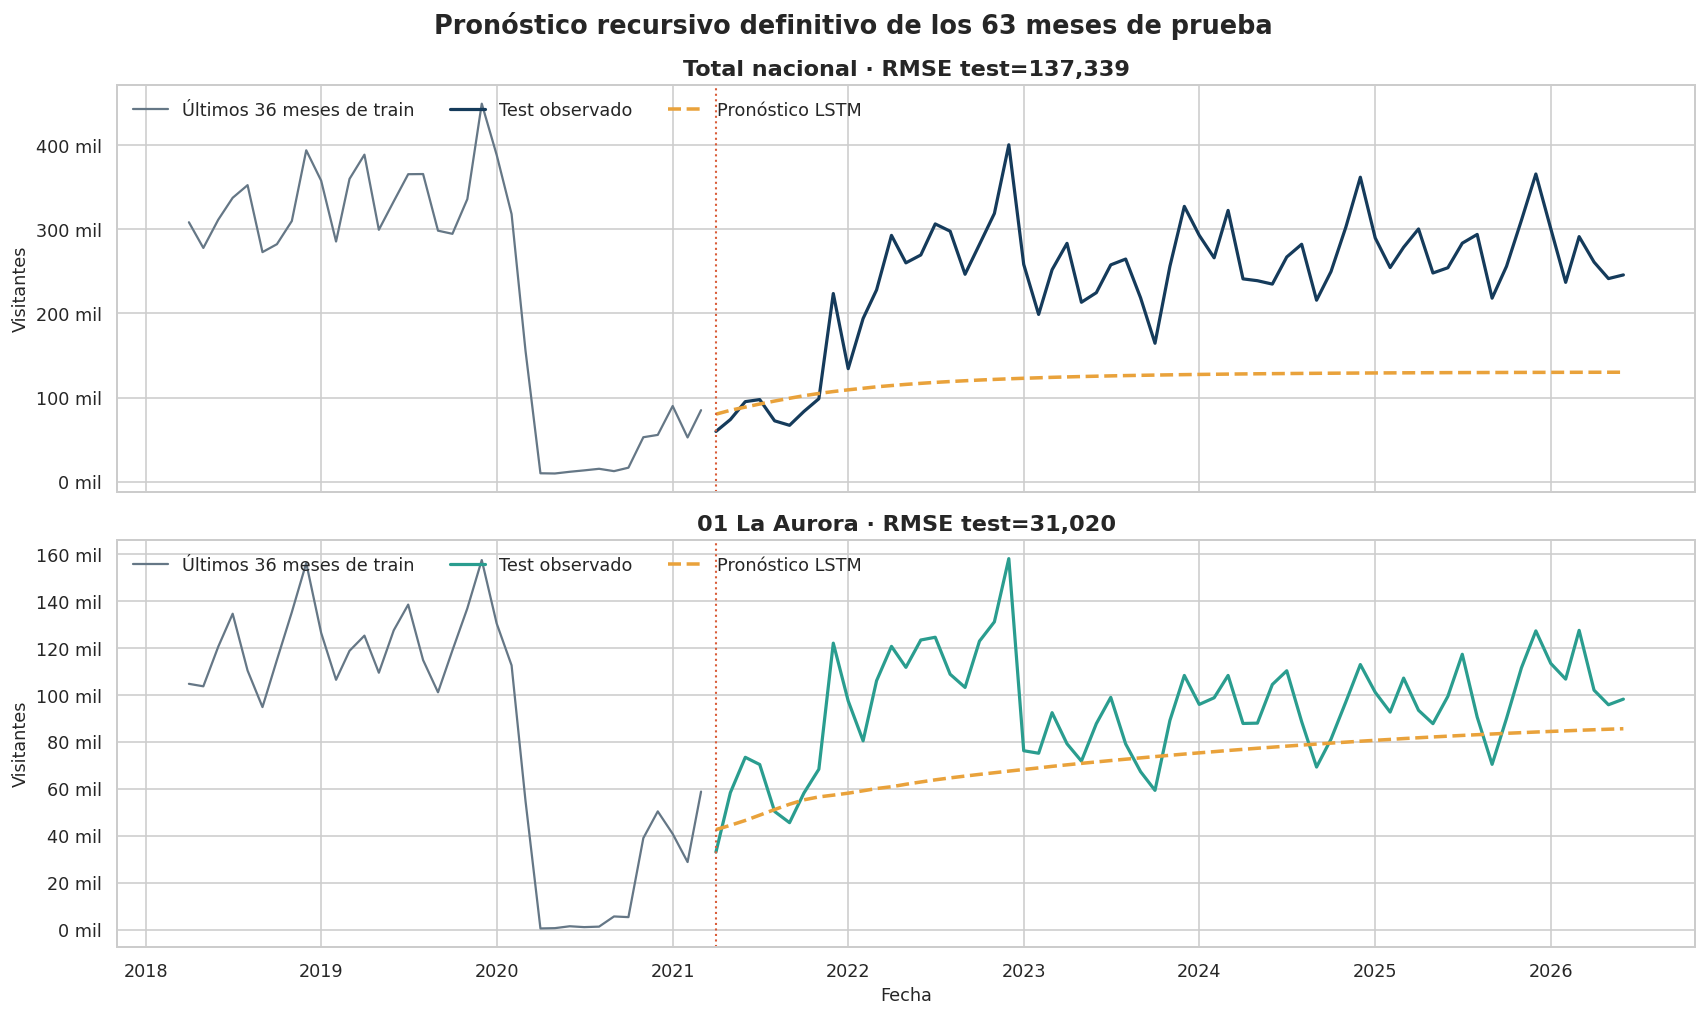
\includegraphics[width=0.98\textwidth]{pronostico_test.png}
\end{center}

En la gráfica, la línea sólida es lo que realmente ocurrió y la línea
punteada es lo que el modelo LSTM estimó para ese mismo período.

\subsection{Total nacional}

El modelo capta bien la recuperación gradual después de la pandemia, pero
luego tiende a ``aplanarse'' más de lo debido: no reproduce cada subida y
bajada mensual. Esto explica por qué su ventaja frente a Prophet fue pequeña
y por qué su error porcentual se mantuvo relativamente alto.

\subsection{La Aurora}

Aquí el pronóstico sigue con más fidelidad el nivel general de visitantes
tras la reapertura de fronteras. No acierta cada pico puntual, pero su
trayectoria general queda más cerca de los datos reales, lo cual coincide con
la mejora más marcada que obtuvo frente a SES.

\subsection{¿Por qué el modelo no acierta cada mes exacto?}

\begin{itemize}
  \item El cierre de 2020 fue un evento extraordinario, sin un antecedente
  parecido en el historial disponible.
  \item El modelo no recibió información sobre vuelos, feriados,
  restricciones migratorias, economía o tipo de cambio.
  \item El horizonte de pronóstico supera los cinco años, y en horizontes
  así de largos los pequeños errores se van acumulando mes tras mes.
\end{itemize}

\callout{Gold}{%
\textbf{Cómo usar estos pronósticos.} Son una herramienta de apoyo para
planificar, no una cifra exacta garantizada. Siempre deben revisarse junto con
información actualizada del contexto.
}

\newpage

% ---------------------------------------------------------------------------
% PÁGINA 7
% ---------------------------------------------------------------------------
\section{catch22: una huella digital para cada serie}

Además de pronosticar, se buscó entender qué series se comportan de manera
parecida. Para ello se utilizó \textit{catch22}.

Puede imaginarse como una \textbf{huella digital formada por 22 números}.
Cada número describe un aspecto distinto:

\begin{itemize}
  \item repetición y dependencia entre meses;
  \item presencia de ciclos;
  \item meses excepcionalmente altos o bajos;
  \item cambios rápidos o lentos;
  \item estabilidad y duración de las fluctuaciones.
\end{itemize}

Se construyeron huellas para siete series:

\begin{itemize}
  \item total nacional;
  \item América Del Centro, América Del Norte y Europa;
  \item La Aurora, Valle Nuevo y San Cristóbal.
\end{itemize}

\begin{center}
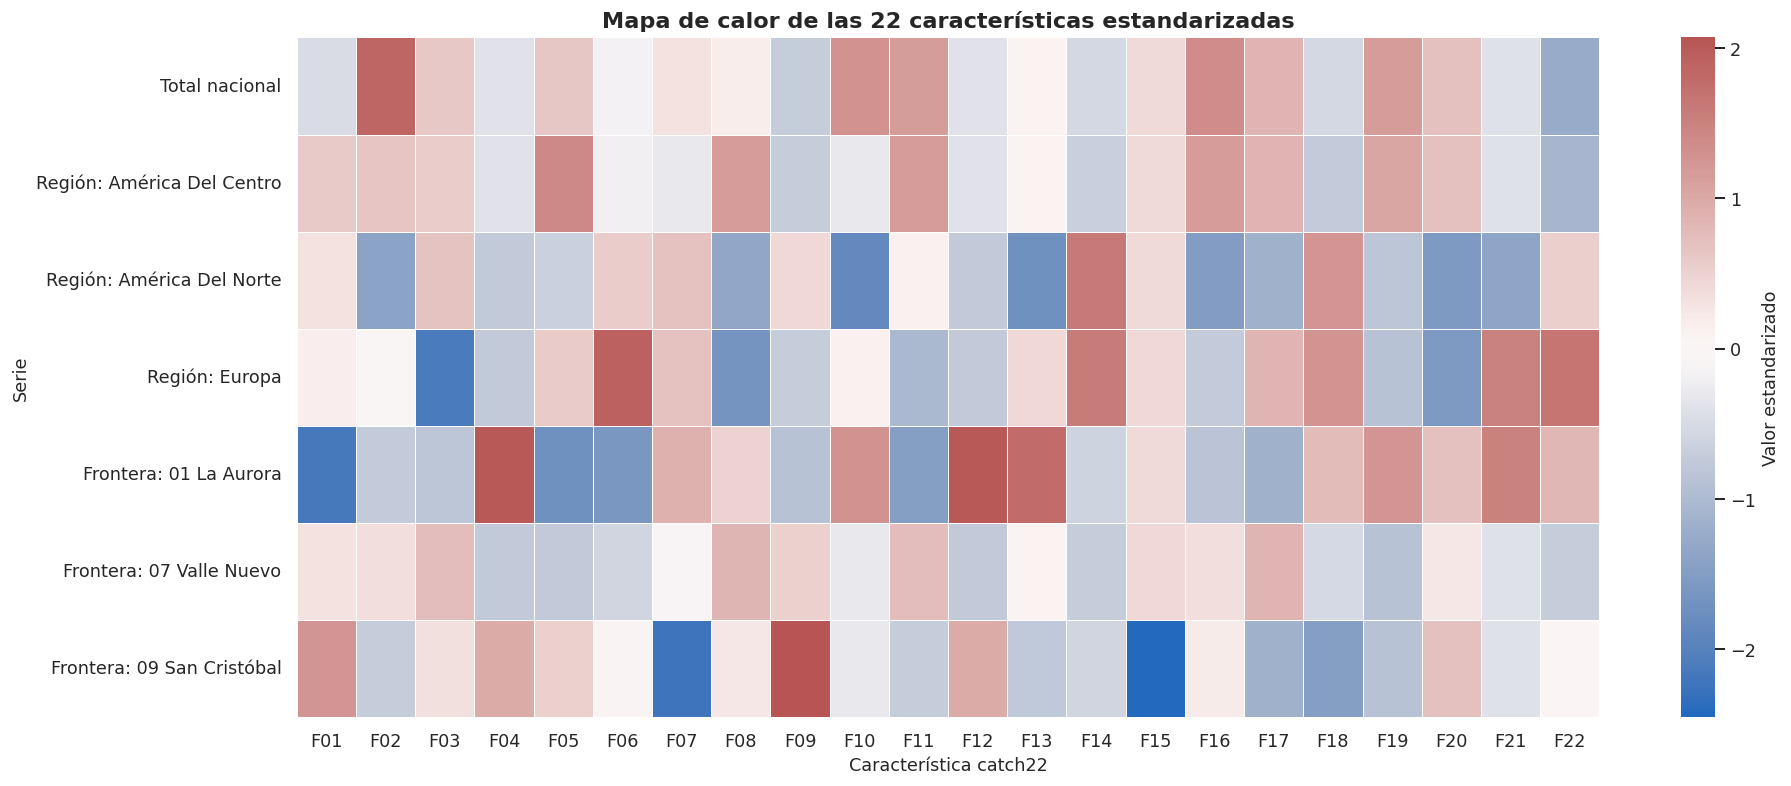
\includegraphics[width=0.98\textwidth]{catch22_heatmap.png}
\end{center}

En el mapa, rojo y azul no significan ``bueno'' o ``malo''. Solamente indican
que una característica está por encima o por debajo del promedio de las siete
series.

\callout{Teal}{%
\textbf{¿Por qué es útil?} Dos series pueden tener cantidades muy diferentes
y, aun así, compartir una forma temporal parecida. catch22 permite estudiar
esa forma sin limitarse al tamaño de los números.
}

\newpage

% ---------------------------------------------------------------------------
% PÁGINA 8
% ---------------------------------------------------------------------------
\section{¿Qué series se parecen?}

El análisis redujo las 22 características a un mapa de dos dimensiones. Los
puntos cercanos representan comportamientos más parecidos.

\begin{center}
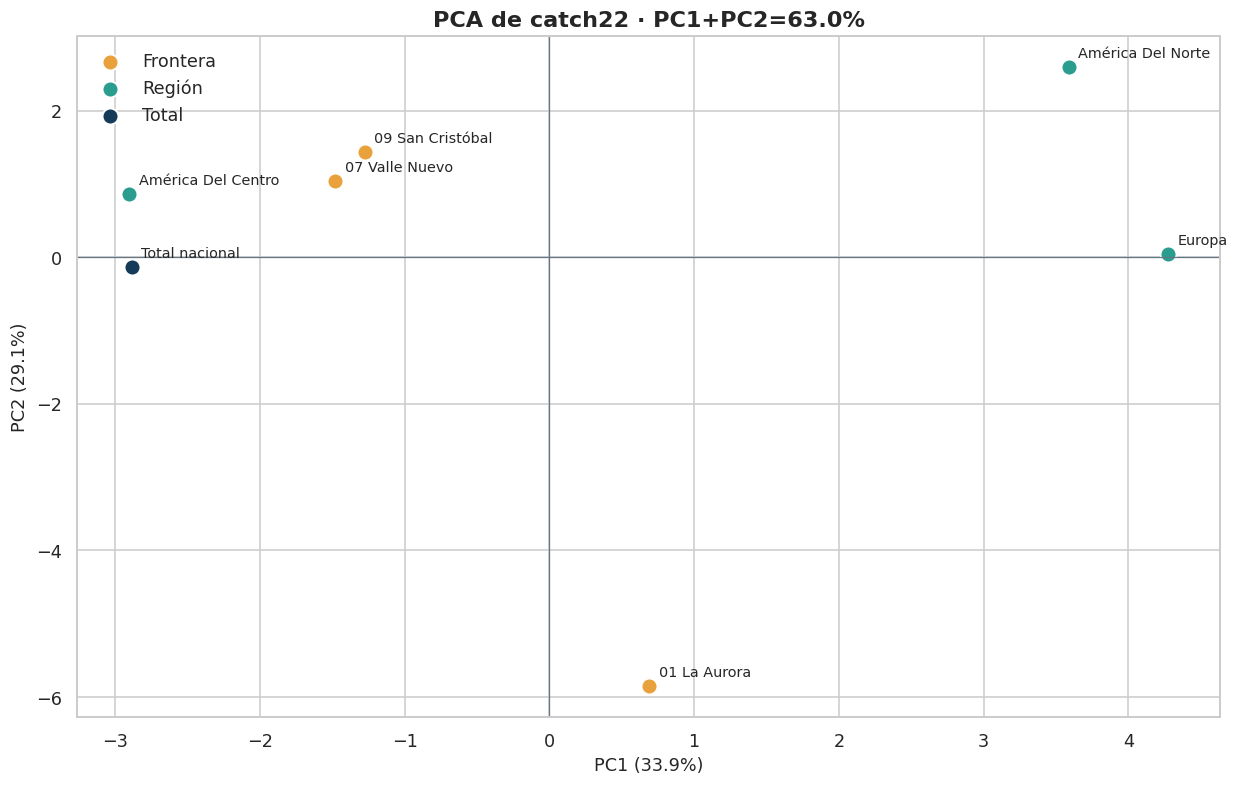
\includegraphics[width=0.73\textwidth]{catch22_pca.png}
\end{center}

\subsection{Resultados más importantes}

\begin{itemize}
  \item \textbf{Par más parecido}: total nacional y América Del Centro.
  \item \textbf{Serie más diferente}: 01 La Aurora.
  \item \textbf{Grupo 1}: total, América Del Centro, Valle Nuevo y San
  Cristóbal.
  \item \textbf{Grupo 2}: América Del Norte y Europa.
  \item \textbf{Grupo 3}: La Aurora por sí sola.
\end{itemize}

La cercanía del total con América Del Centro concuerda con la importancia de
los mercados centroamericanos y las fronteras terrestres. La Aurora se
separa porque depende de vuelos y tuvo una caída y una recuperación
particulares.

\subsection{Un descubrimiento importante}

Pertenecer a la misma categoría no garantiza comportarse igual. La Aurora,
Valle Nuevo y San Cristóbal son fronteras, pero La Aurora no se agrupa con las
otras dos. La forma en que cambia una serie a lo largo del tiempo puede ser
más informativa que su etiqueta administrativa.

\callout{Gold}{%
El análisis utiliza únicamente siete series. Los grupos son una guía
exploratoria y no una clasificación permanente de todas las fronteras o
mercados.
}

\newpage

% ---------------------------------------------------------------------------
% PÁGINA 9
% ---------------------------------------------------------------------------
\section{¿Agregar catch22 mejoró la predicción?}

Se construyó un último modelo para La Aurora. Además de observar los 12 meses
recientes, recibió la huella catch22 calculada con los 36 meses anteriores.

\begin{center}
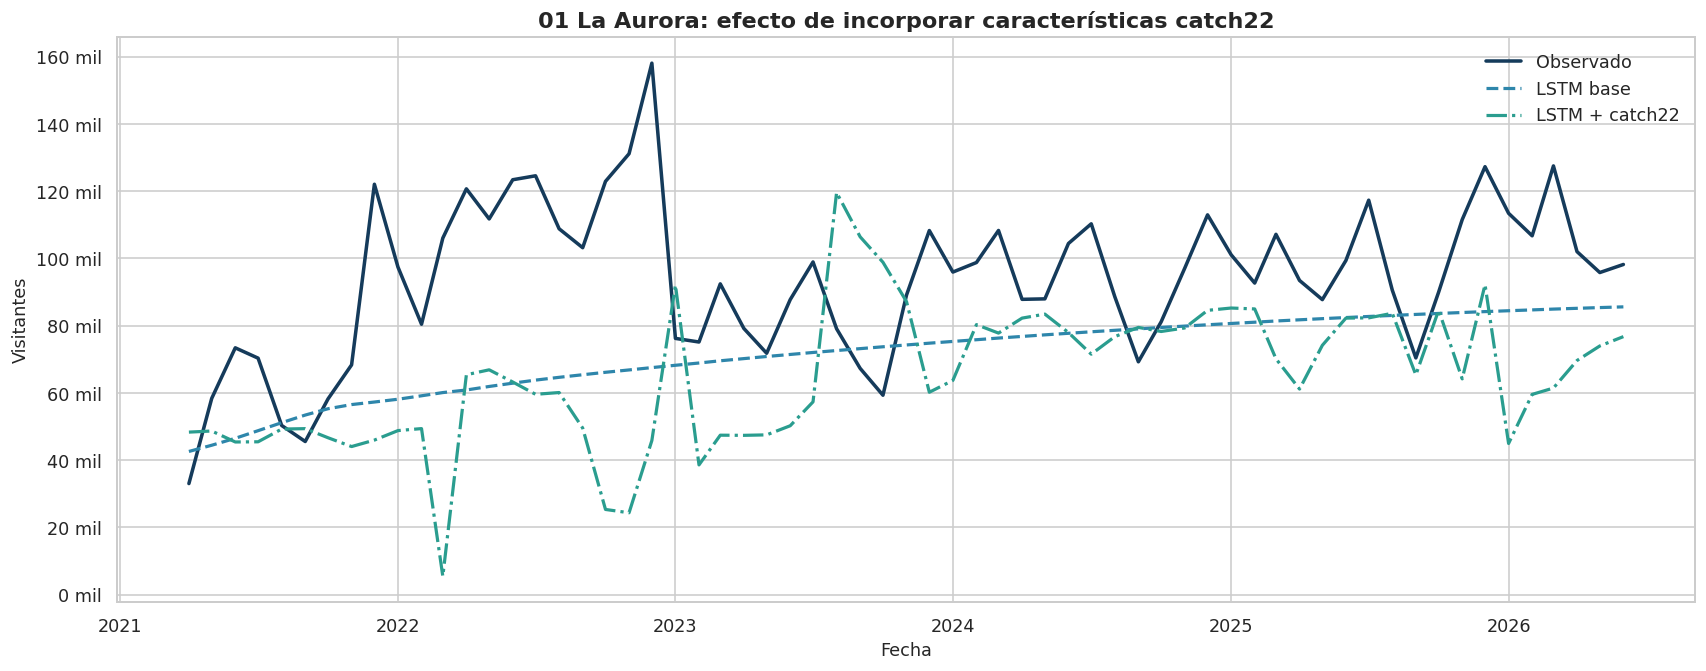
\includegraphics[width=0.93\textwidth]{lstm_catch22.png}
\end{center}

\begin{tabularx}{\textwidth}{Xrr}
\toprule
\textbf{Modelo} & \textbf{MAE} & \textbf{RMSE}\\
\midrule
LSTM base & 24,473 & \textbf{31,020}\\
SES & 36,822 & 42,053\\
LSTM con catch22 & 34,356 & 42,907\\
\bottomrule
\end{tabularx}

\subsection{El resultado fue negativo, pero útil}

La versión con catch22 \textbf{no mejoró} la predicción. Su RMSE fue 42,907,
frente a 31,020 de la LSTM base. Agregar más información hizo el modelo más
complejo, pero no más preciso.

Esto puede ocurrir porque:

\begin{itemize}
  \item había pocos ejemplos para aprender 23 entradas al mismo tiempo;
  \item varias características contenían información repetida;
  \item una huella que sirve para comparar series completas no
  necesariamente ayuda a pronosticar cada mes.
\end{itemize}

\callout{Teal}{%
\textbf{Aprendizaje obtenido.} Un resultado que no mejora también es
importante. Evita adoptar una solución más complicada cuando la versión
sencilla funciona mejor.
}

\newpage

% ---------------------------------------------------------------------------
% PÁGINA 10
% ---------------------------------------------------------------------------
\section{Conclusiones y recomendaciones}

\subsection{Conclusiones principales}

\begin{enumerate}
  \item Se analizaron 210 meses completos y dos series de visitantes.
  \item Se probaron cuatro versiones LSTM por cada serie.
  \item La LSTM redujo el error de La Aurora en 26.24\% frente a SES.
  \item En el total nacional la mejora frente a Prophet fue de 1.58\%.
  \item El total y América Del Centro fueron las series más parecidas.
  \item La Aurora fue la serie con comportamiento más particular.
  \item Agregar catch22 a la LSTM no mejoró el pronóstico.
\end{enumerate}

\subsection{Recomendaciones para uso práctico}

\begin{itemize}
  \item Actualizar los modelos cuando se incorporen meses nuevos.
  \item Mantener varios métodos disponibles; no imponer un único algoritmo.
  \item Separar pronósticos por frontera o región cuando se planifiquen
  recursos locales.
  \item Incorporar vuelos, feriados, restricciones y variables económicas.
  \item Presentar intervalos o escenarios, no solamente una cifra puntual.
  \item Documentar cualquier cambio en la forma de registrar visitantes.
\end{itemize}

\subsection{Glosario mínimo}

\begin{tabularx}{\textwidth}{>{\bfseries\color{Blue}}p{2.8cm}X}
LSTM & Método que aprende patrones en datos ordenados y conserva memoria de
meses anteriores.\\
Pronóstico & Estimación de un valor que todavía no se conoce.\\
RMSE & Medida de error que penaliza más las equivocaciones grandes.\\
catch22 & Conjunto de 22 números que resume la forma temporal de una serie.\\
PCA & Mapa simplificado para observar semejanzas entre muchas
características.\\
Clustering & Procedimiento que reúne elementos con comportamientos
parecidos.\\
\end{tabularx}

\callout{Teal}{%
\textbf{Mensaje final.} Los modelos pueden apoyar decisiones, pero deben
combinarse con conocimiento institucional y datos recientes. La LSTM base fue
la opción más efectiva para las dos series evaluadas.
}

\vfill
{\small\color{Navy}
\textbf{Nota:} resultados académicos; no constituyen cifras oficiales ni un
sistema institucional de pronóstico.}

\end{document}
